\setchapterpreamble[u]{\margintoc}
\chapter{Technical details}
\labch{practical}

Bringing all previous theoretical concepts into a working model is not straightforward if approached from scratch but, since the late 2000s and early 2010s, there have been notable advancements in programming libraries which take care of the hard work of calculating gradients and optimizing weights, leaving to the data scientist just the task of designing an appropriate model.

This chapter is dedicated to illustrating the reader on the different possibilities that exist for designing and implementing autoencoder networks. Detailed examples on how to code simple autoencoders are provided.

\section{Design}

Designing an autoencoder for a certain task can be challenging, since the objective is to find a more useful representation of the data but we cannot know the size of the optimal representation beforehand, thus difficulting decisions about the number of layers and the size of each one.

\subsection{Type of layers}

Different layers are available in every deep learning framework and can be used according to the structure of the provided data and the kind of operations the practitioner wants to apply to it.

\begin{itemize}
    \item \textbf{Unstructured variables}: the most basic type of data takes the form of tabular values where columns may be related but do not hold a specific structure, they can be reordered in any way and the data is still valid. Appropriate layers for this kind of data are dense layers, also known as fully connected or linear. These compute a product between the input vector and a matrix of parameters, which gives a new output vector as a result.
    \item \textbf{Images}: the recent surge in deep learning applications is in great part due to the potential of convolutional operations for image processing. These relieve a great part of the computational complexity of dense layers by leveraging the spatial relations among values. This is done by computing new values out of multiplying parameters with a neighborhood of input values, thus not taking into account the whole image for each individual value in the output. Convolutional layers are frequently coupled with pooling layers (either max-pooling or average-pooling) which reduce the dimensionality of the data points, as well as dropout layers which randomly disable some layer nodes during training in order to improve model robustness.
    \item \textbf{Sound, time series and sequential data}: there exist many data sources which impose a one-dimensional structure to the values, e.g. recorded sounds, stock prices, sensor signals across time, etc. Convolutional operations can also apply in this case, since they can operate in one dimension analogously to the two-dimensional version. However, other layers have been specifically designed for this kind of data, such as long short-term memory (LSTM) units or gated recurrent units (GRU). These are encompassed under the term \textit{recurrent units}.
\end{itemize}

\subsection{Model depth}

Determining how deep a model should become, i.e., how many layers to stack, is a process influenced by the amount of variables and instances in the dataset. Taking into account that deep learning models are usually data-hungry, defining a model with many layers will require a large dataset in order to optimize all parameters. This inconvenience is especially present in the case of dense layer-based models, since these have many more parameters than convolutional models.

\subsection{Encoding layer}

Autoencoders being mainly feature learners, the most important layer is that where the new representation of the data will be extracted. Some aspects that are important to evaluate are the dimension or shape of the encoding and the activation function.

The dimension of the encoding layer will determine the compactness of the new representation. Thus, if the objective is to find a small set of variables for a dataset, a short length will be selected for this layer. The optimal size can be hard to find, but if the layer is too small the behavior of the autoencoder will generally be poor (the loss function will not decrease during training) so a practical way of estimating an appropriate size is to start with a very short layer and increase the size until the training process is able to converge.

For its part, the activation function will determine the range of the values that will be obtained. This is relevant if, for instance, bounded values are needed for a later purpose. In that case, a sigmoid or a $\tanh$ activation function would be helpful in providing values within the $[0,1]$ and $[-1,1]$ ranges, respectively.

\subsection{Output layer}

Finally, the output layer needs to preserve the same structure of the input data. This means that, if an instance is composed of $n$ values, this layer needs to produce $n$ outputs.

It is also convenient to consider the range of the input values if an activation is to be applied to the final layer. 
Using the appropriate activation function in the output layer can facilitate the reconstruction task of the autoencoder. 
\begin{itemize}
    \item \textbf{Unbounded}: for data with unbounded variables, no activation (also known as "linear" activation in some frameworks) is the adequate decision, since most activations restrict the range of the output.
    \item \textbf{Partially bounded}: Nonnegative data can be generated by a ReLU activation.
    \item \textbf{Bounded interval}: Data in the $[0,1]$ range can be produced as the result of a sigmoid activation. Similarly, the $\tanh$ activation function can provide data in the $[-1,1]$ range.
\end{itemize}

\section{Implementation}

During the latest years, there has been a notable evolution in the scene of software libraries for deep learning. From the existence of a wide variety of them with differing functionalities, ease of use and optimizations, there has been a tendency to condensate popularity in just two of them, which currently offer very similar functionalities and interfaces: Tensorflow and Pytorch.

\begin{figure*}[htbp]
    \centering  
    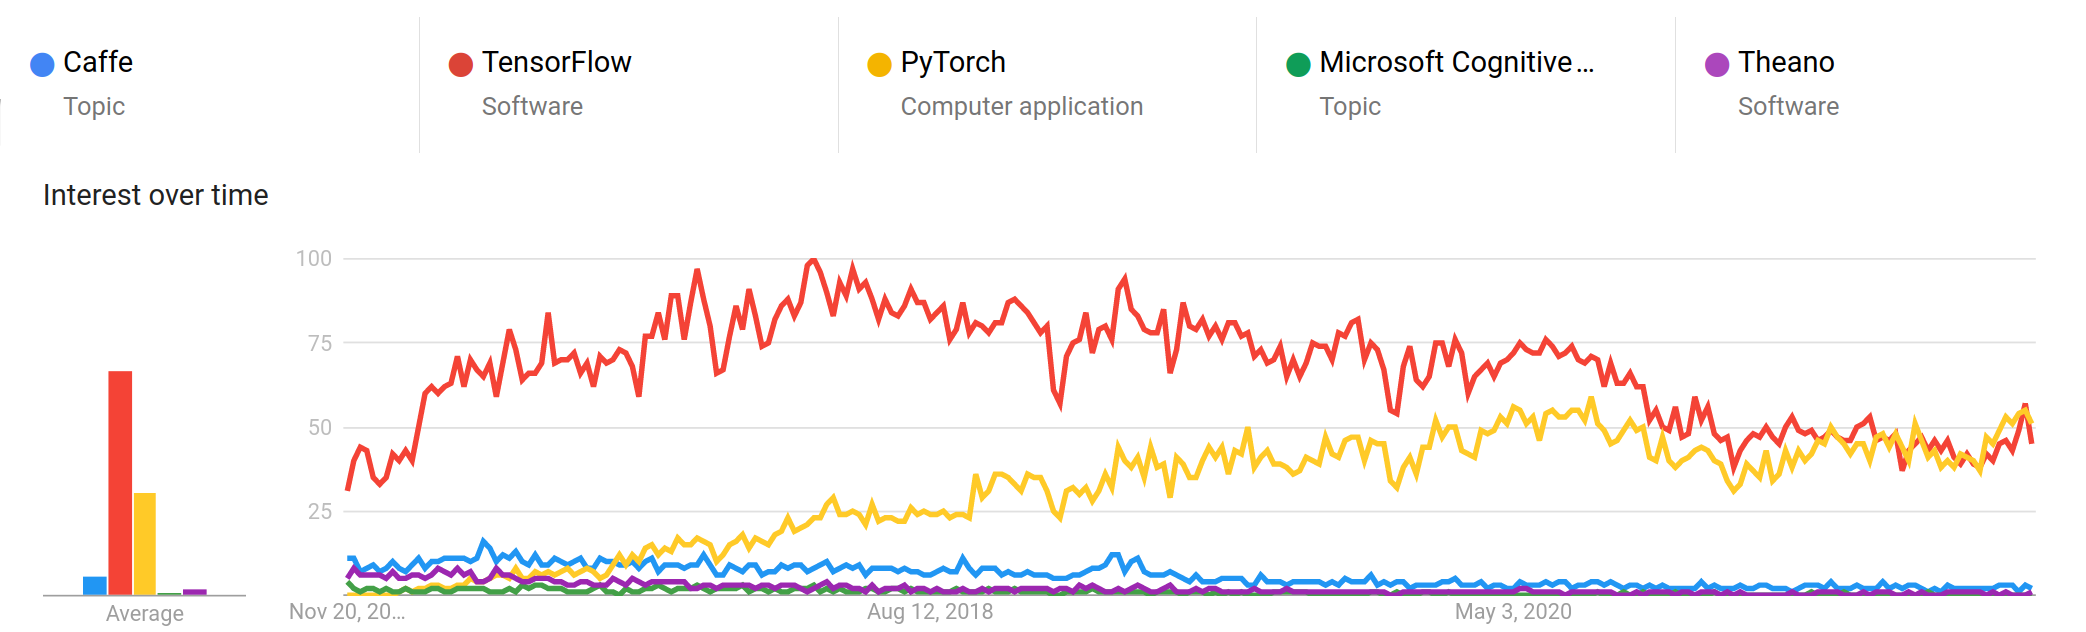
\includegraphics[width=\linewidth]{library_trends.png}
    \caption{Trends for web searches for five of the most popular deep learning frameworks, over the last 5 years.}
    \label{fig:trends}
\end{figure*}

\subsection{About Tensorflow}

Tensorflow is a deep learning framework implemented in C++, with Python and C++ interfaces, developed by Google and open source contributors.

This library provides both lazy and eager execution of tensor operations on either CPU or GPU. Eager execution, the usual way of running statements where the result of each statement is readily available just after an operation is run, is enabled by default starting from Tensorflow 2. Lazy execution behaves the opposite, delaying the actual computation of operations until a final step where everything is processed jointly. It allows to optimize models better using a computation graph, but makes it harder to debug them.

Tensorflow integrates an easy-to-use API called Keras \sidecite{keras}, which raises the level of abstraction so that the user does not need to program each operation but can design a network based on its layers. This API also brings additional tools including prebuilt and pretrained models, data manipulation functionalities, built-in datasets and automatic parameter tuning.

\subsubsection{Sample implementation}

Consider an essential autoencoder model where both the encoder and the decoder are composed of one fully connected layer. 

For the purpose of modularity, which helps reusing parts of the code later, it is convenient to define the encoder and the decoder separately. Each will be represented by an object of class \texttt{Sequential}, and comprises a list with just one layer, of class \texttt{Dense}. 

Both models are chained by listing them in a new \texttt{Sequential} model, which is then compiled to optimize the binary crossentropy loss using the Adam \sidecite{Adam} optimizer. Assuming that the variable \texttt{x\_train} holds the training data, the model is optimized when the \texttt{fit()} method is called.

Once the autoencoder has been trained, the encoder can be fed new instances from the same variable space and it will map those to the learned representation.

\begin{lstlisting}[language=Python]
import tensorflow as tf

enc_dim = 10
encoder = tf.keras.Sequential([
    tf.keras.layers.Dense(enc_dim, activation="relu", 
        input_shape=(x_train.shape[1], ))
])
decoder = tf.keras.Sequential([
    tf.keras.layers.Dense(x_train.shape[1], 
        activation="sigmoid", input_shape=(enc_dim,))
])

autoencoder = tf.keras.Sequential([encoder, decoder])
autoencoder.compile(loss="binary_crossentropy", 
    optimizer="adam")
autoencoder.fit(x_train, x_train, epochs=10)

new_encodings = encoder.predict(x_test)
\end{lstlisting}

\subsection{About Pytorch}

Pytorch is the successor of the Lua-based Torch library, with the objective of providing an interface as natural as possible for the experienced Python user. It is developed by Facebook and other open source contributors.

This library attempts to provide a deeper integration with Numpy and Scipy, and is designed to work in eager execution but models can be transformed into graph mode (which enables lazy execution and further optimizations).

The Pytorch API is well organized into modules depending on the type of data that is being processed: \texttt{torchvision} for images, \texttt{torchaudio} for audio sequences and \texttt{torchtext} for text and natural language. Models can be built in a similar fashion to the Keras interface, but the training process usually requires more explicit code.

\subsubsection{Sample implementation}

Next is an equivalent implementation for the same autoencoder of the previous example, this time in Pytorch. The similarities can be appreciated when defining the encoder and the decoder, but the optimization of the autoencoder model is done more explicitly this time, by means of a training loop. At each iteration, the following steps are performed:

\begin{enumerate}
    \item A batch of input samples is selected
    \item The neural network is feeded these samples and its output is obtained
    \item A loss metric is calculated according to the target outputs
    \item The gradients applied to the model are reset
    \item The gradients corresponding to the current loss are computed and propagated
    \item Model parameters are updated by the optimizer according to the gradients
\end{enumerate}

Once the training loop has finished, the model is considered trained and is switched to evaluation mode in order to allow for extraction of the learned features for new data.

\begin{lstlisting}[language=Python]
import torch
from torch.nn.functional import binary_cross_entropy

enc_dim = 10

encoder = torch.nn.Sequential(
    torch.nn.Linear(x_train.shape[1], enc_dim),
    torch.nn.ReLU(True)
)
decoder = torch.nn.Sequential(
    torch.nn.Linear(enc_dim, x_train.shape[1]),
    torch.nn.ReLU(True)
)

autoencoder = torch.nn.Sequential(encoder, decoder)

optimizer = torch.optim.Adam(autoencoder.parameters())

for i in range(100):
    inputs = x_train[i*10:(i+1)*10]
    output = autoencoder(inputs)
    loss = binary_cross_entropy(output, inputs)
    autoencoder.zero_grad()
    loss.backward()
    optimizer.step()

autoencoder.eval()
encoder(x_test)
\end{lstlisting}

\section{Training deep models}

The training process of a deep learning model can be very resource-intensive, since it requires computing hundreds of arithmetic operations, usually across several thousands of parameters. 

\subsection{GPU parallelization}
